
\section{Introduction}\label{sec:AnalysisStrategy_Intro}
The search for a new resonance $X$ is described in this chapter.

The main production mode for the Higgs boson particle over the all mass spectrum is the gluon-gluon fusion (ggH) process. At a center-of-mass energy of 13\TeV the ggH cross section for a Higgs boson mass ($m_\mathrm{H}$) of 125\GeV is 43.92\,pb~\cite{temphiggsxsecs}, that is almost one order of magnitude larger than the second process  in terms of cross section at that mass, VBF, with 3.748\,pb~\cite{temphiggsxsecs}. The  gluon-gluon fusion cross section decreases with $m_\mathrm{H}$ but the VBF/ggH cross section ratio increases with the mass, making the VBF production mechanism more and more important as $m_\mathrm{H}$ approaches to high values.\\
The signal samples are interpreted in terms of the EWK singlet model described in Sec~\ref{sec:signalModel} below. 
The Higgs boson width and lineshape is reweighted at generator level according to the parameters defined in the model.
The interference effects between the ggH signal, the ggWW background and SM
Higgs boson, that are expected to slightly change the lineshape of the signal
distribution, have been fully taken into account, as detailed in
Sec.~\ref{sec:interference}. A similar treatment is also applied for the
intereference between the VBF high mass signal, the VBF SM Higgs and the quark
initiated WW+2 quarks backgrround. The interference between the $\mathrm{W^+W^-}\to2\ell2\nu$ and $\mathrm{ZZ}\to2\ell2\nu$ is negligible due to the different phase space characteristic of these processes. 


The analysis strategy for the high mass search with 2016 data in the
$\mathrm{W^+W^-}\to2\ell2\nu$ decay channel  is similar to the previous high
mass analysis with 2015 data~\cite{CMS-PAS-HIG-16-023}, but has several improvements. \\
The analysis is divided in two parts: 
\begin{itemize}
\item the opposite-flavour final state, $e^{\pm} \mu^{\mp}$,
\item the  same-flavour final state, $e^+ e^-$ and  $\mu^+ \mu^-$. 
\end{itemize}
In the opposite-flavour final state four different jets-categories are defined: the 
0-jet, the 1-jet, the 2-jet non VBF and finally the VBF. The 2-jet non-VBF category is new with respect to previous analysis with 2015 data.\\
In the same-flavour final state only the VBF category is considered. Indeed, the only the VBF selection cuts are sufficiently tight to reduce the  overwhelming Z+jets background to a manageable level.




\section{Discriminating variable}
This analysis is a shape analysis, meaning that after
applying selection cuts we do not simply count events, but rather we fit a data histogram of a
discriminating variable with the sum of signal and background templates, and
extract the signal yield from the fit.
The variable with the best discriminating value would be the invariant mass of
the four lepton, which is not possible to reconstruct in the \WW channel due
to neutrinos.\\
For the Higgs boson in \WW analysis, the shape analysis is based on two-dimensional templates of $m_{\ell \ell}$ versus $m_T^H$, where  the transverse mass  $m_T^H$ variable is defined as  
\begin{equation}
 m_T^H = \sqrt{2p_{\rm T}^{\ell\ell}\MET(1-\mathrm{cos}\Delta\phi(\ell\ell, \ptvecmiss))}
\end{equation}
where $\Delta\phi(\ell\ell, \ptvecmiss)$ is the azimuthal angle between the dilepton momentum and \ptvecmiss.\\
However  $m_T^H$ (and also $m_{\ell \ell}$) is not very sensitive to the
signal mass hypothesis, so a \textit{new} variable $m_T^I$ defined as the visible mass,
\begin{equation}
 m_T^I = \sqrt{ (p_\mathrm{\ell\ell} + \MET)^2 - (\vec{p}_\mathrm{\ell\ell} + \ptvecmiss)^2 }
\end{equation}
has been introduced  to discriminate better the high mass $X$ signals generate at different masses.
The distribution of the variables defined above are shown in
Fig.~\ref{fig:mt_nocuts}, where it is visible the better power of $m_T^I$ in discriminating
different mass hypotheses respect the other variable.

\begin{figure}[htbp]
\centering
\subfigure[True generated mass]{
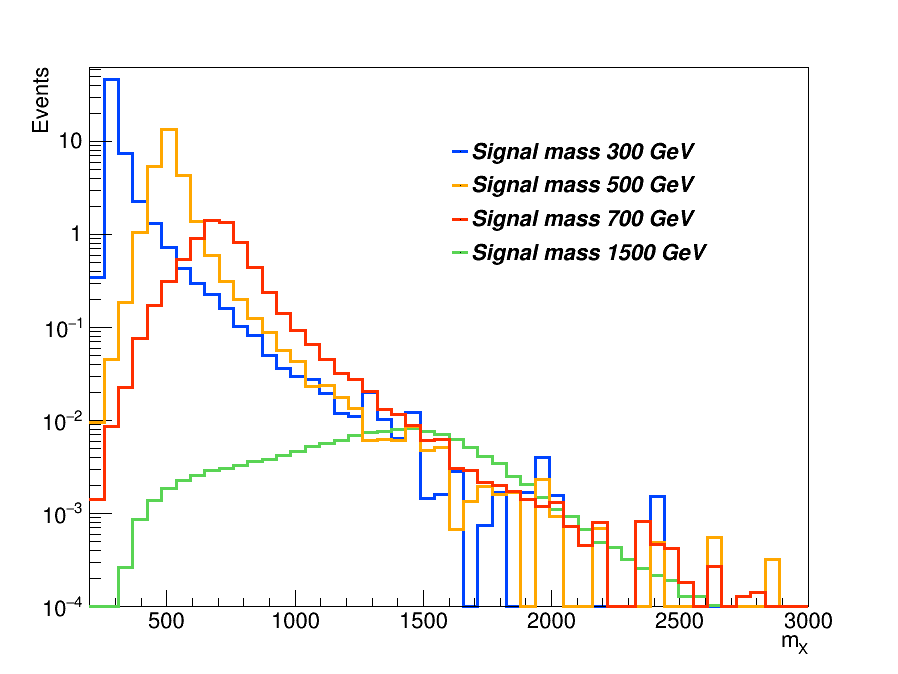
\includegraphics[width=0.45\textwidth]{../AN/Figs/Distribution_higgsLHEmass_cuts_nocuts.png}
}
\subfigure[$m_T^H$]{
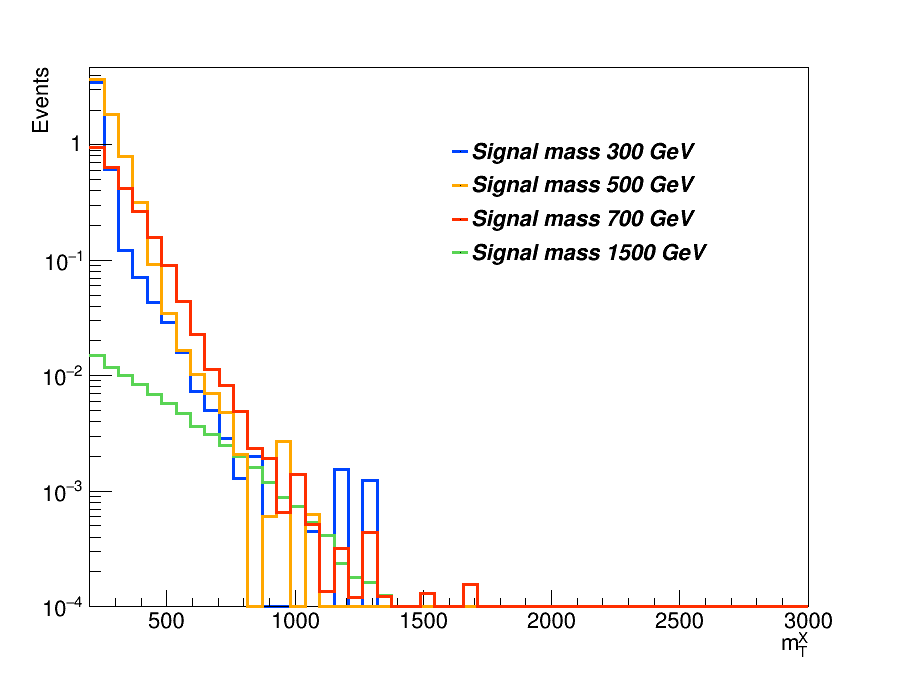
\includegraphics[width=0.45\textwidth]{../AN/Figs/Distribution_mth_cuts_nocuts.png}
}
\\
\subfigure[$m_{\ell \ell}$]{
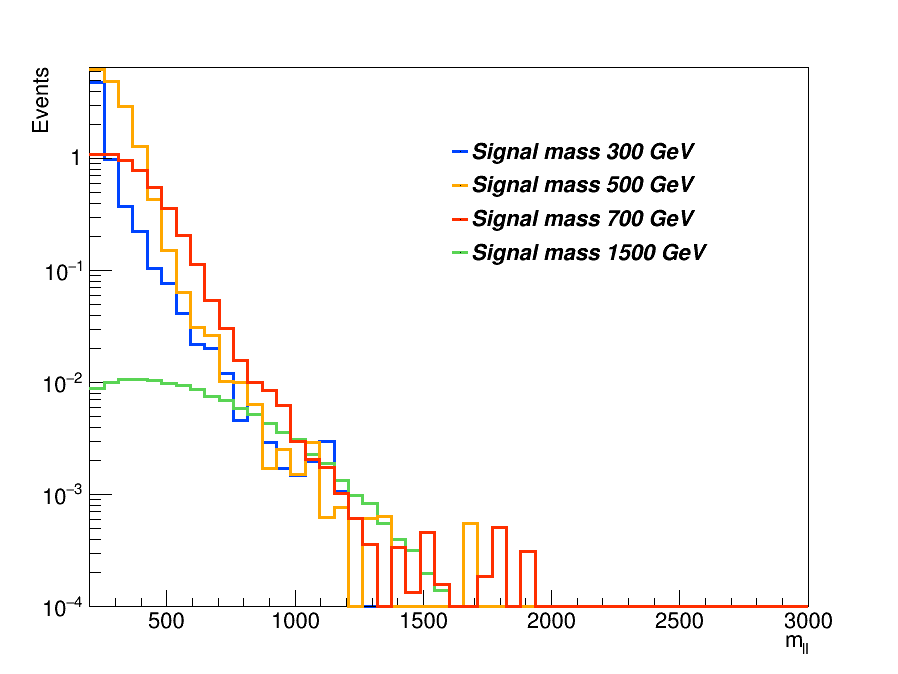
\includegraphics[width=0.45\textwidth]{../AN/Figs/Distribution_mll_cuts_nocuts.png}
}
\subfigure[$m_T^I$]{
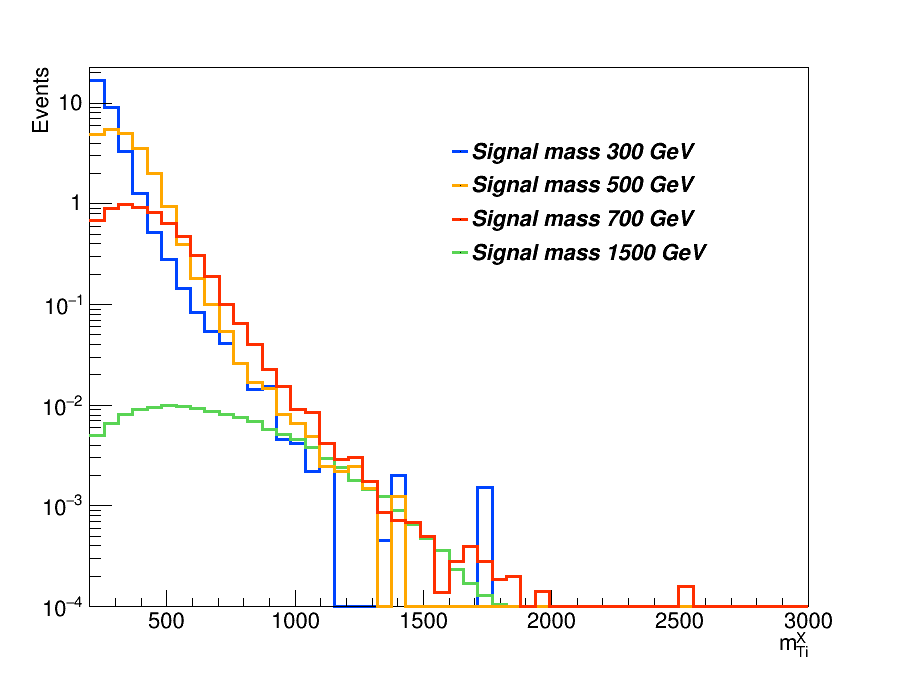
\includegraphics[width=0.45\textwidth]{../AN/Figs/Distribution_mTi_cuts_nocuts.png}
}
\caption{
    Distributions of the generated mass, $m_T^H$, $m_{\ell \ell}$ and  $m_T^I$
    variables for different $X$ mass hypothesis.}
    \label{fig:mt_nocuts}
\end{figure}

%#################


\section{Signal interpretation}
\label{sec:signalModel}
The signal is interpreted in terms of the electroweak singlet model, representing a scalar mixing with the 125\GeV Higgs boson. This model relies on two parameters: the scale factor of the couplings of the high mass resonance with respect to the SM, $C'$, and the branching fraction of the electroweak singlet to non-SM decays modes, $BR_\mathrm{new}$. The electroweak singlet signal strength, $\mu'$ and the modified width, $\Gamma'$, are related with the parameters in the model by the following equations:

\begin{equation}
\mu' = C'^2 \cdot (1 - BR_\mathrm{new})
\end{equation}
\begin{equation}
\Gamma' = \Gamma_\mathrm{SM} \cdot \frac{C'^2}{1 - BR_\mathrm{new}}
\end{equation}

The available Higgs signal samples for different mass hypothesis have been reweighted according to this model. At the moment only the $BR_\mathrm{new} = 0$ hypothesis has been investigated while we tested different $C'$ values.
In Fig.~\ref{fig:cprime} are shown the \mll and \mt templates corresponding to a Higgs boson mass of 700\GeV for three different $C'$ values: $C' = 1$, corresponding to the SM Higgs decay width, $C'=0.5$, corresponding to $\Gamma' = 2.5\cdot10^{-2}\,\Gamma_\mathrm{SM}$, and $C'=0.1$, corresponding to $\Gamma' = 10^{-2}\,\Gamma_\mathrm{SM}$. A value of $BR_\mathrm{new} = 0$ is considered in all cases. We note that the signal shape is not very sensitive to different $C'$ values.

\begin{figure}[htbp]
\centering
\subfigure[Simulated LHE signals]{
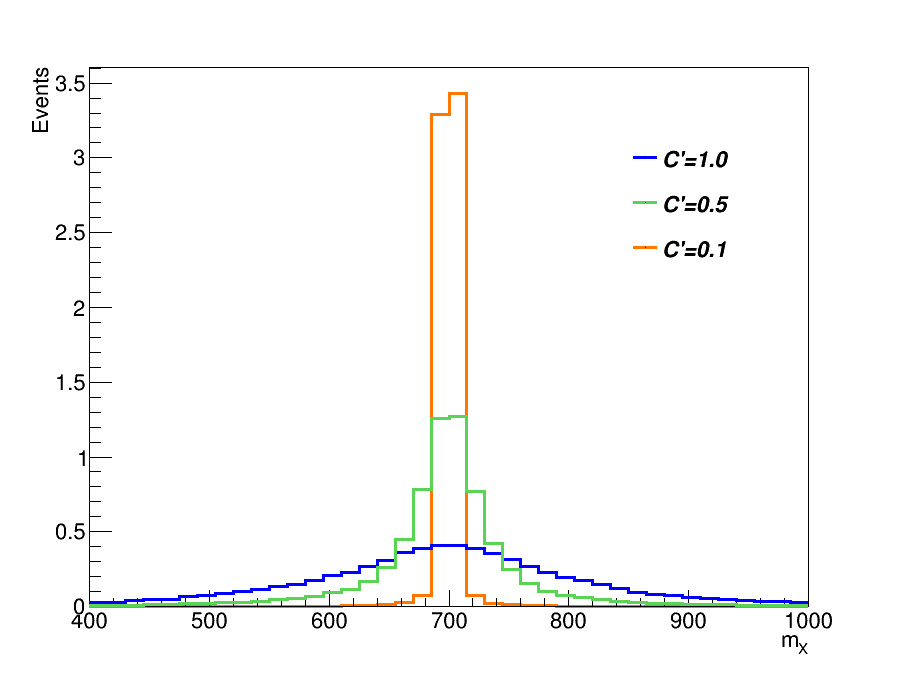
\includegraphics[width=0.45\textwidth]{../AN/Figs/higgsLHEmass700_cuts_nocuts.png}
}
\subfigure[$m_T^H$]{
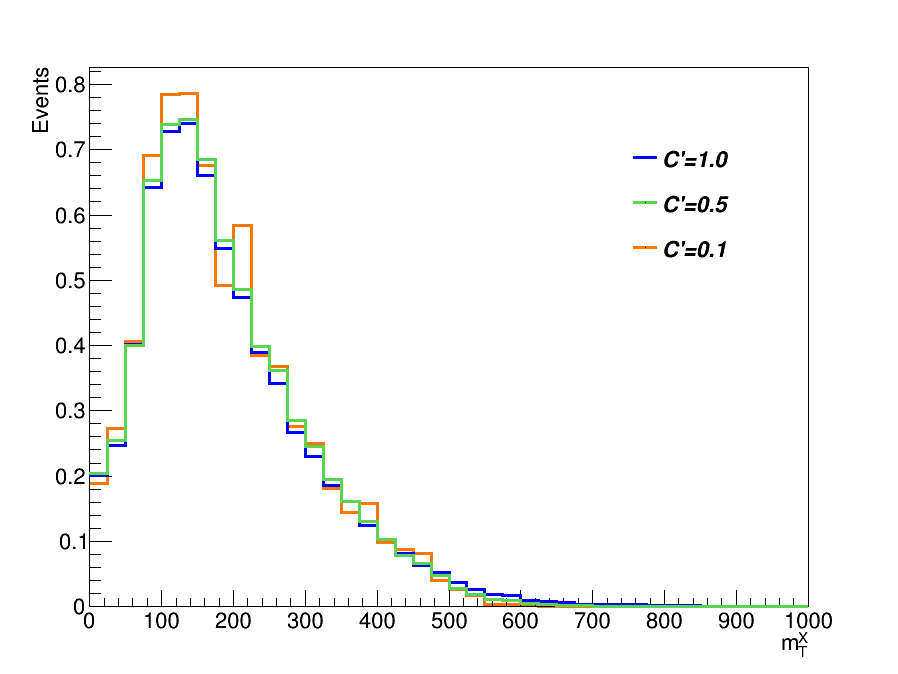
\includegraphics[width=0.45\textwidth]{../AN/Figs/mth700_cuts_nocuts.png}
}
\\
\subfigure[$m_{\ell \ell}$]{
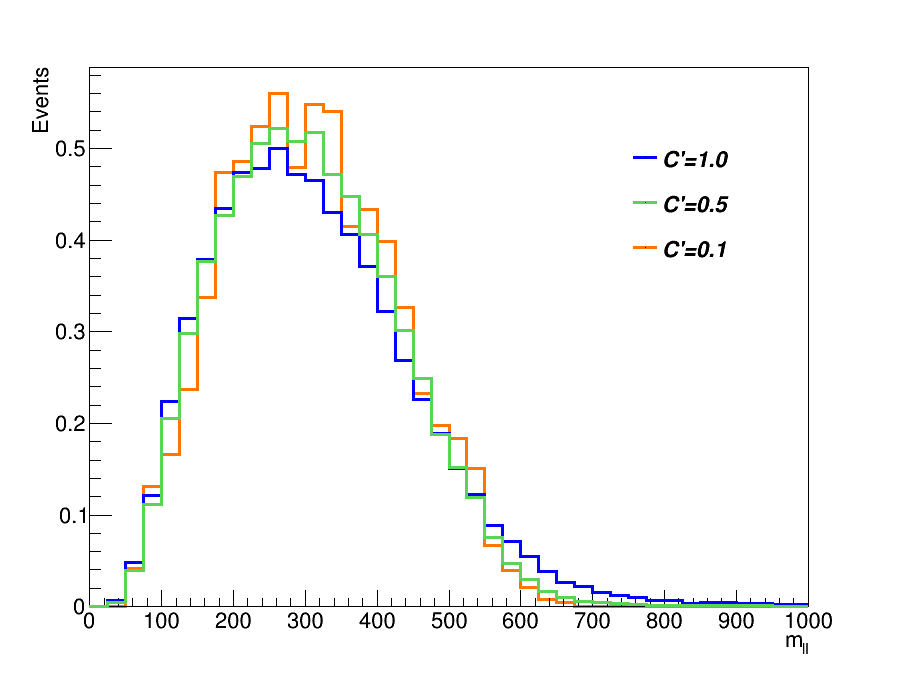
\includegraphics[width=0.45\textwidth]{../AN/Figs/mll700_cuts_nocuts.png}
}
\subfigure[$m_T^I$]{
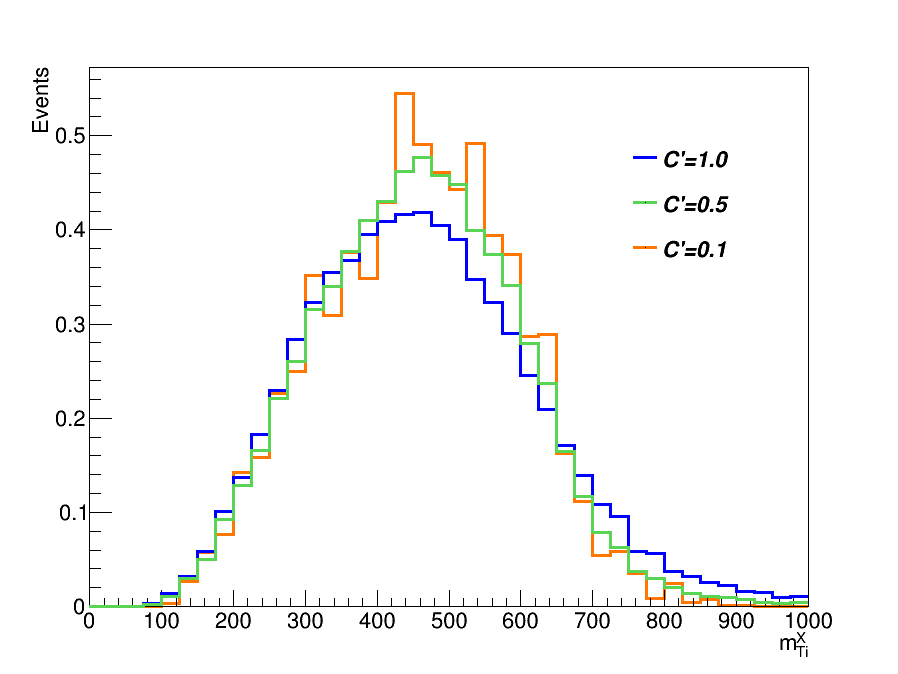
\includegraphics[width=0.45\textwidth]{../AN/Figs/mTi700_cuts_nocuts.png}
}
\caption{ 
    Distributions of the signals, the $m_T^H$, the $m_{\ell \ell}$ and the  $m_T^I$ variables at generator level for different values of $C'$, without any selection.}
    \label{fig:cprime}
\end{figure}



\subsection*{Study of the Interference effects}
\label{sec:interference}
When a resonance $X$, with a non negligible width is considered, it is important to take into account also the interference effects both with the \WW background , with same initial and final state, and with the Higgs boson off-shell tail. 

In this analysis  we take into account the interference effects between the
new signal X produced in gluon-gluon fusion and in vector-boson-fusion.
The effect of the various interference terms are shown in ~\ref{fig:X300} and  \ref{fig:Int_VBF_GEN} for the two different production mechanism, gluon-gluon fusion and vector-boson.fusion.  The contribution of the interference of $X$ with \WW background  and with Higgs boson have opposite sign and partially cancel out. This cancellation effect is different for different resonance masses.
The interference contribution is thus non negligible and is included in the fit. \\
%To prevent possible negative probability distribution function of the interference,  during the fit the signal yield is computated as,
%\begin{equation}
%Yield=\sqrt{\mu} \times (S+B+I)+ (\mu -\sqrt{\mu}) \times (S) + (1-\sqrt{\mu}) \times (B)
%\end{equation}
%where  $S$ is the signal, $B$ the background and $I$ the interference.


\begin{figure}[htbp]
\centering
\subfigure[Mass 300 \GeV.]{
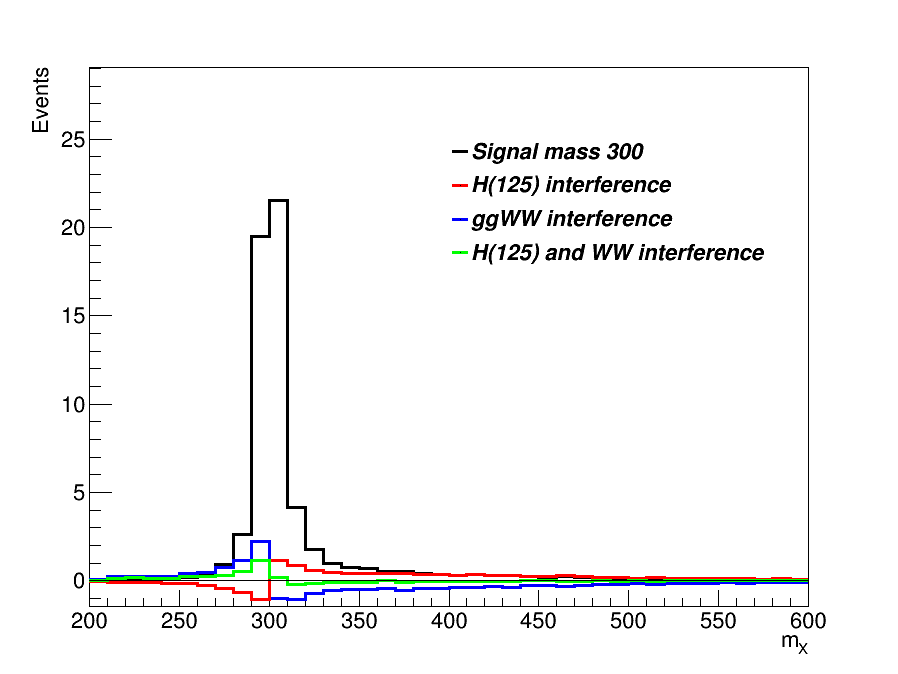
\includegraphics[width=0.45\textwidth]{../AN/Figs/Interference_higgsLHEmass300_cuts_nocuts.png}
}
\subfigure[Mass 400 \GeV.]{
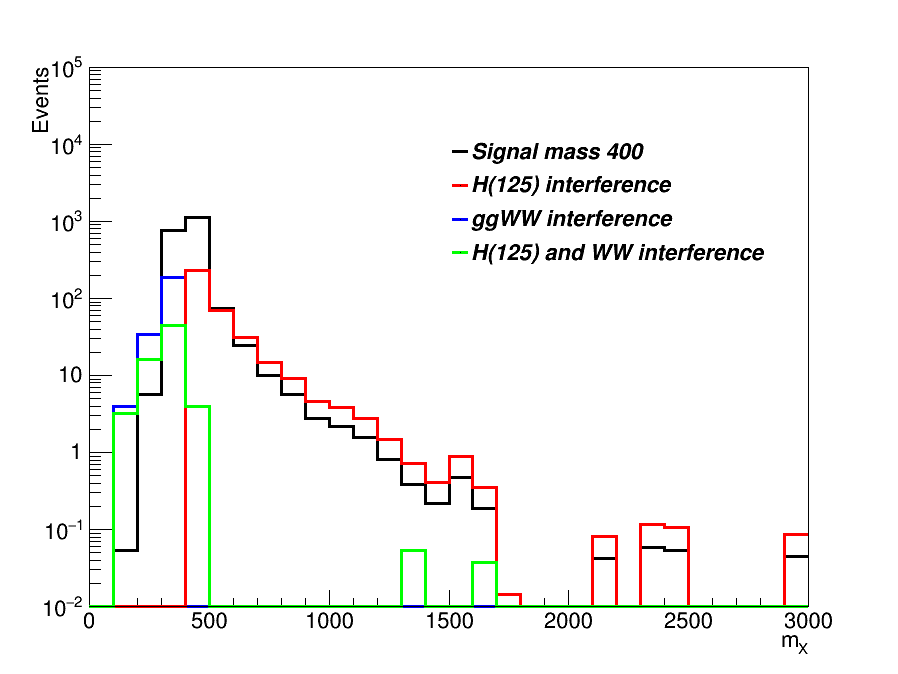
\includegraphics[width=0.45\textwidth]{../AN/Figs/Interference_higgsLHEmass400_cuts_nocuts.png}
}
\\
\subfigure[Mass 700 \GeV.]{
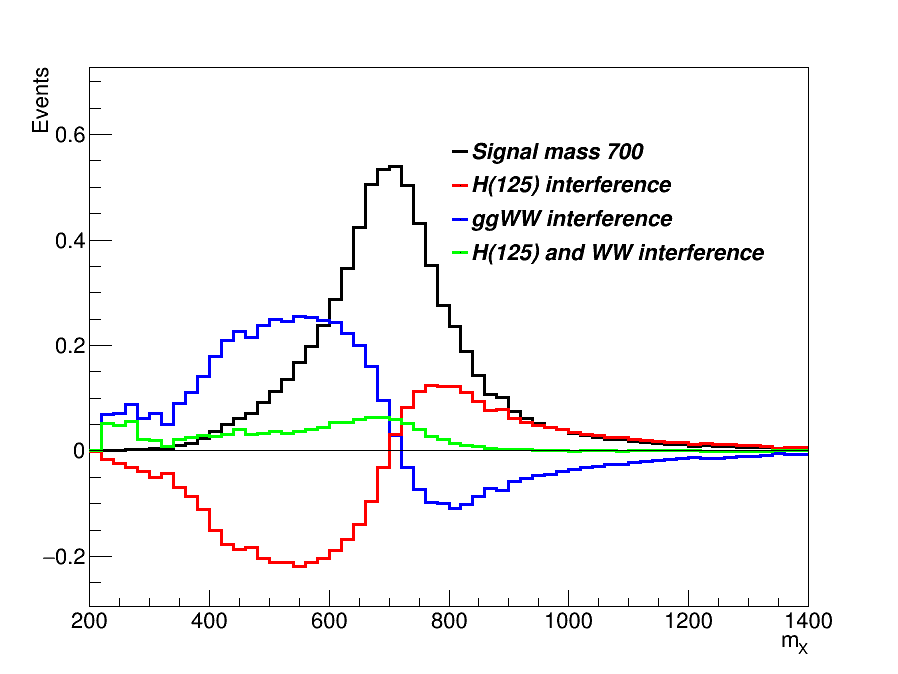
\includegraphics[width=0.45\textwidth]{../AN/Figs/Interference_higgsLHEmass700_cuts_nocuts.png}
}
\subfigure[Mass 1500 \GeV.]{
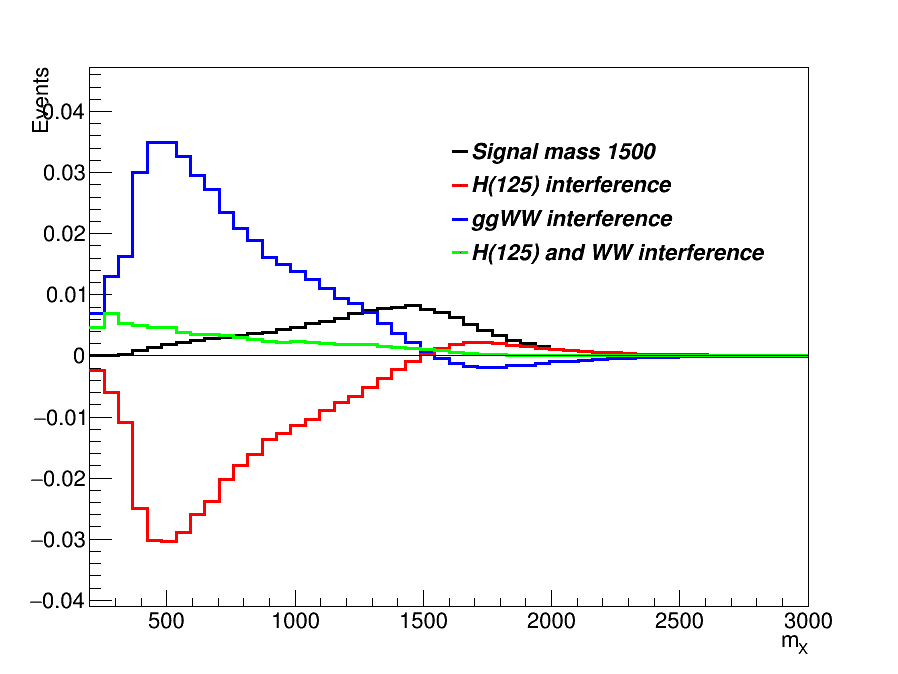
\includegraphics[width=0.45\textwidth]{../AN/Figs/Interference_higgsLHEmass1500_cuts_nocuts.png}
}
\caption{Distribution of for the $X$ mass resonance, produced via gluon-gluon fusion for different masses. In black the high mass signal. In red the interference between the high mass signal and the Higgs boson. In blue the interference between the high mass signal and the background. In green the total interference i.e. high 
mass signal, Higgs bison and background. }
    \label{fig:X300}
\end{figure}





\begin{figure}[htbp]
\centering
\subfigure[Mass 300 \GeV]{
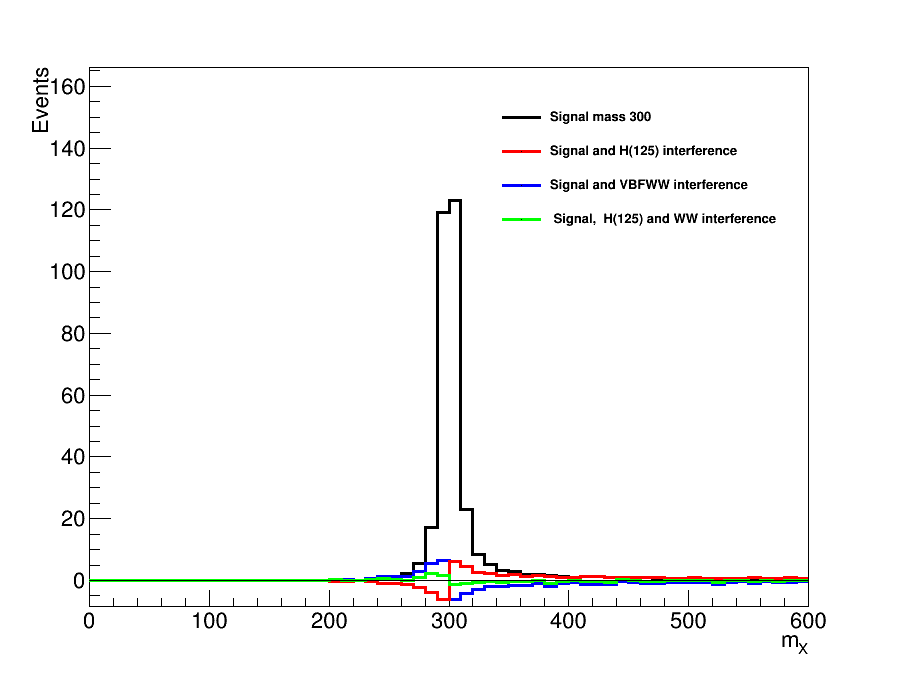
\includegraphics[width=0.45\textwidth]{../AN/Figs/Inter_VFB/Interference_higgsLHEmass300_cuts_nocuts.png}
}
\subfigure[Mass 1500 \GeV]{
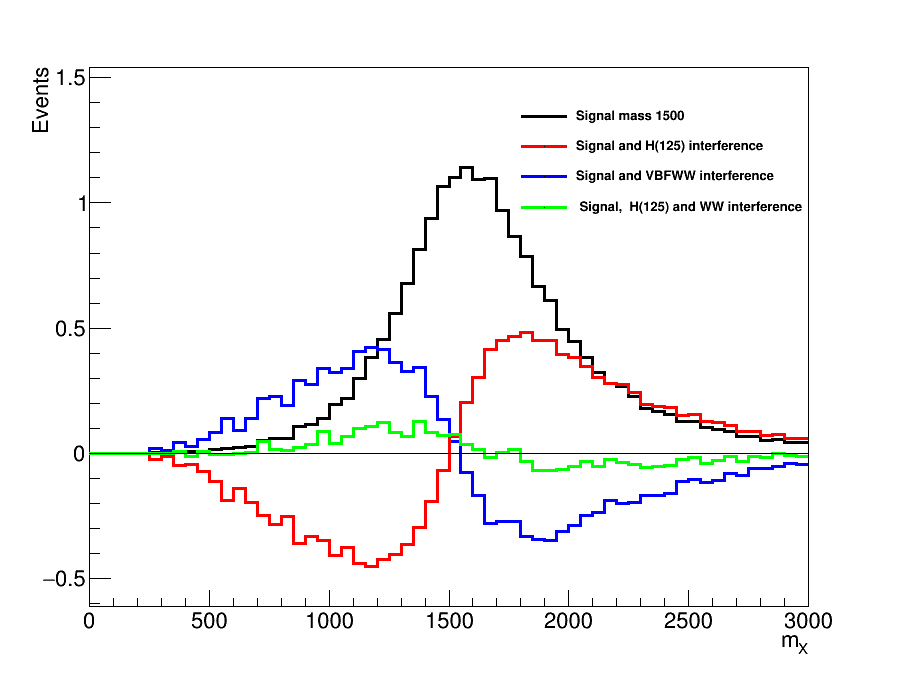
\includegraphics[width=0.45\textwidth]{../AN/Figs/Inter_VFB/Interference_higgsLHEmass1500_cuts_nocuts.png}
}
\caption{Distribution of for the $X$ mass resonance, produced via vector-boson-fusion fusion for different masses. In black the high mass signal. In red the interference between the high mass signal and the Higgs boson. In blue the interference between the high mass signal and the background. In green the total interference i.e. high 
mass signal, Higgs bison and background.}
    \label{fig:Int_VBF_GEN}
\end{figure}









































